 \chapter{Theory of Kerr frequency combs in Fabry-Perot resonators} \label{chap:FPLLE}
 
 \begin{footnotesize}
 \begin{spacing}{1.2}
 	This chapter describes work that was reported in:
 	\begin{itemize}
 		\item \fullcite{Cole2018a}.\\
 	\end{itemize}
 \end{spacing}
\end{footnotesize}

Generation of Kerr frequency combs in the ring-resonator geometry appears quite promising for applications. However, a second possibility is to use the same processes for comb generation, but with a Fabry-Perot (FP) resonator geometry. The FP geometry offers a new degree of freedom relative to the ring resonator, which is the possibility to employ chirped mirrors, mirror coatings, or distributed Bragg reflectors, and therefore exert greater control over the total cavity dispersion. Other differences with the ring geometry may ultimately prove important; for example, the smaller footprint possible in a cavity of total length $L$ with the FP geometry versus the ring geometry could allow for denser and more flexible integration of Kerr combs in photonics systems. Kerr-comb generation in an FP cavity was reported in 2009 in Ref. \citeNoBrackets{Braje2009} and soliton generation using a pulsed pump laser was recently described in Ref. \citeNoBrackets{Obrzud2017}.

In this chapter we present a brief theoretical investigation of the difference in the nonlinear dynamics that occur in a Kerr-nonlinear FP resonator versus a Kerr-nonlinear ring resonator. Our starting point is the Fabry-Perot Lugiato-Lefever equation (FP-LLE), which is derived in detail in Ref. \citeNoBrackets{Cole2018a}, beginning from a set of coupled equations that describe the interaction of the envelopes for the forward- and backward-propagating fields in the cavity with the Kerr medium. A derivation of equivalent coupled mode equations is provided in Ref. \citeNoBrackets{Obrzud2017}. We do not reproduce the derivation of the equation here; our goal is to understand its description of Kerr-comb dynamics. The equation is:
\begin{equation}
\frac{\partial\psi}{\partial\tau}=-(1+i\alpha)\psi+i|\psi|^2\psi-i\frac{\beta_2}{2}\frac{\partial^2\psi}{\partial\theta^2}+2i\psi\left<|\psi|^2\right>+F\label{eq:FPLLE}.
\end{equation}
Here, $<g>$ denotes the spatial average over the domain: $<g>=\frac{1}{2\pi}\int_{-\pi}^{\pi}d\theta\,g(\theta)$. This equation is identical to the LLE for the ring cavity except for the term $2i\psi\left<|\psi|^2\right>$ describing modulation by twice the average of the intracavity power. The coordinate $\theta$ is defined as $\theta=\pi z/L$, where $z$ is a co-moving longitudinal coordinate (so that, for example, solitons are stationary functions of $\theta$) on a domain $-L\leq z\leq L$; $L$ is the single-pass length of the Fabry-Perot cavity. The time $\tau$ is once again normalized to twice the photon lifetime $\tau_{ph}$: $\tau=t/2\tau_{ph}$. The normalized experimental parameters in the FP-LLE are the same as in the LLE for the ring cavity, with $\alpha$ the detuning, $\beta_2$ the dispersion, and $F^2$ the pump power:
\begin{equation}
\alpha=-\frac{2(\omega_o-\omega_c)}{\Delta\omega_o},
\end{equation}
\begin{equation}
\beta_2=\left.-\frac{2D_2}{\Delta\omega_{tot}}=-\frac{2}{\Delta\omega_o}\frac{\partial^2\omega_\mu}{\partial \mu^2}\right|_{\mu=0}, \label{betaLLE}
\end{equation}
\begin{equation}
F^2=\frac{8g_o\Delta\omega_{ext}}{\Delta\omega_{tot}^3}\frac{A_{eff}}{A_{in}}\frac{n_o}{n_{ext}}\frac{P}{\hbar\omega_o}.
\end{equation}
In the above, $\omega_\mu$ represents the set of resonance frequencies of the cavity including the effects of dispersion, with $\mu=0$ indexing the pumped mode. The cavity loss and coupling rates $\Delta\omega$ and $\Delta\omega_{ext}$ are related to the mirror reflectivity $R$ and transmission $T$ via $\Delta\omega=(1-R)c/n_gL$ (where two identical mirrors are assumed) and $\Delta\omega_{ext}=cT/2n_gL$, with $n_g=c/v_g$ the group index. The quantities $A_{in}$ and $A_{eff}$ represent the mode's effective area $\pi w_{in}^2$ (for a Gaussian mode of radius $w$) at the input mirror and the same averaged over the cavity of length $L$, $\frac{\pi}{L}\int dz\, w(z)^2$, respectively. Further, $g_0=n_2\hbar\omega_o^2 D_1/(2\pi n_g A_{eff})$ is the nonlinear gain parameter, where $D_1=\left.\frac{\partial\omega_\mu}{\partial \mu}\right|_{\mu=0}$ is the cavity free-spectral range in angular frequency (here and in Eq.~(\ref{betaLLE}) $\mu$ is treated as a continuous variable). The nonlinear index $n_2$ is related to the third-order susceptibility via $\chi^{(3)}=(4/3)n_0^2\epsilon_0cn_2$, where $n_0$ is the refractive index of the nonlinear medium.  The power $P=\eta P_{inc}$ denotes the mode-matched power, with mode-matching factor $\eta$ and power $P_{inc}$ incident on the input mirror, and $n_{ext}$ is the refractive index of the medium external to the cavity. 

\begin{figure}[htpb]
	\begin{center}
		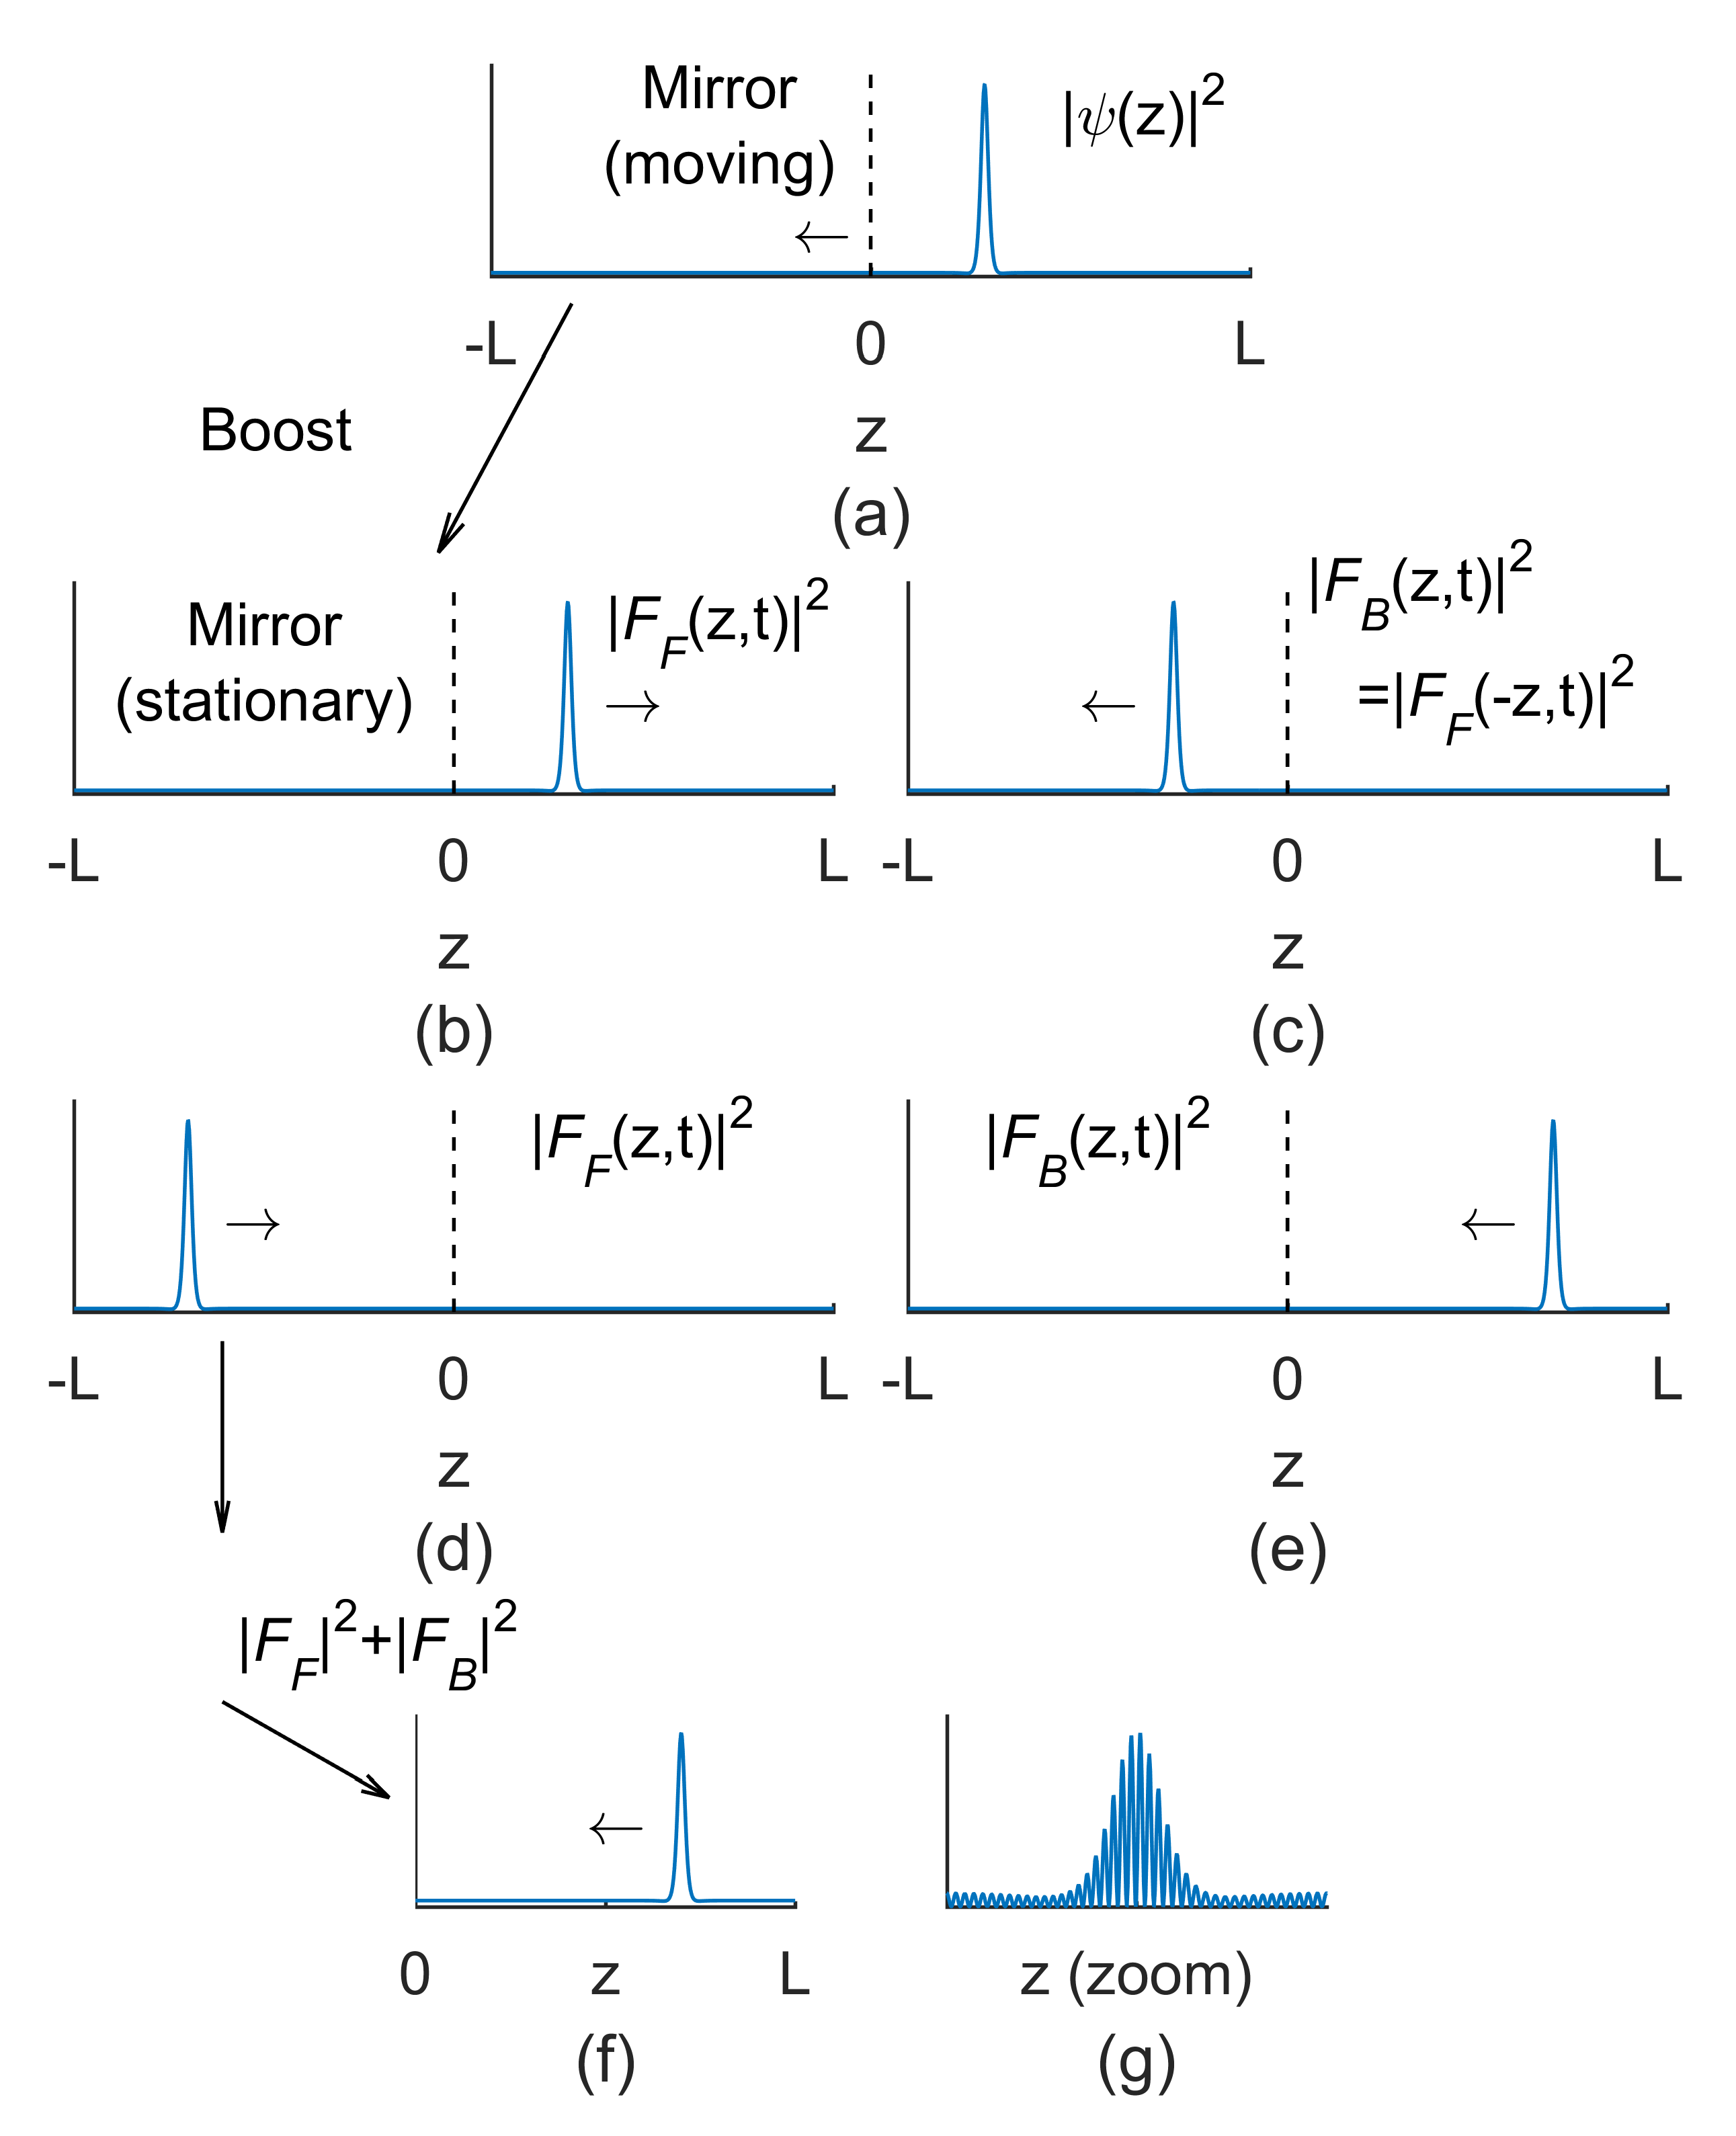
\includegraphics[]{\FigPath/Figures/FPLLE/FPLLEfieldconstruction.png}
	\end{center}
	\caption[Relationship between the physical field in the Fabry-Perot cavity and the co-moving field $\psi$]{\textbf{Relationship between the physical field in the Fabry-Perot cavity and the co-moving field $\psi$.} (a) A soliton stationary solution to the FP-LLE in the co-moving domain of length $2L$, in which the physical components of the cavity (e.g. mirror) move. (b) Intensity of the field $F_F$ in the lab frame, in which the cavity is stationary. (c) Intensity of $F_B$ in the lab frame, related to $F_F$ by reflection about the origin. (d,e) Depictions of the same after propagation for half of the cavity round-trip time. (f) Total intensity of the field on the physical domain $0 \leq z \leq L$. (g)~The intensity of the field including the background standing wave that results multiplication of $F_F$ and $F_B$ by the appropriate traveling waves. }
	\label{fig:FPLLEfieldconstruction}
\end{figure} 

The formulation of the FP-LLE in terms of the field $\psi$ defined in the co-moving domain of length $2L$ facilitates numerical simulation of the nonlinear dynamics. To obtain the physical, propagating field in the Fabry-Perot cavity, the arguments of the field $\psi$ are transformed back to dimensionful parameters so that we have $\psi(z,t)$, and then this field is boosted to group velocity $v_g$ in the domain of length $2L$ to obtain $\psi_v$, which propagates with periodic boundary conditions $\psi_v(-L,t)=\psi_v(L,t)$. From $\psi_v(z,t)$ we define functions $F_F$ and $F_B$ that are proportional to the forward-propagating and backward-propagating envelopes of the electric field as $F_F(z,t)\propto\psi_v(z,t)$ and $F_B(z,t)\propto\psi_v(-z,t)$, so that they are related by reflection about $z=0$. The quantity $|F_B(z,t)|^2+|F_F(z,t)|^2$ on the physical domain $0\leq z \leq L$ is then proportional to the intensity in the FP cavity as a function of time, averaged over fast spatial and temporal oscillations associated with the optical frequency. If desired, these can be included by multiplying $F_B$ and $F_F$ by the appropriate traveling waves before summation. This process is depicted schematically in Fig. \ref{fig:FPLLEfieldconstruction}.



In the remainder of this chapter we provide an investigation of the nonlinear dynamics in a Fabry-Perot cavity as they relate to the generation of frequency combs.

\section{General relationship between the ring LLE and the FP-LLE}
As can be seen from Eq. \ref{eq:FPLLE} for the Fabry-Perot cavity and Eq. \ref{eq:LLE} for the ring cavity, the difference between the two geometries lies in the term in the FP-LLE $2i\psi\left<|\psi|^2\right>$. This term represents the cross-phase modulation of the field $\psi(\theta,\tau)$ at each co-moving point $\theta$ by the field $\psi(\theta',\tau)$ at each other co-moving point $\theta'$ as $\theta$ and $\theta'$ propagate through each other during a round trip of the Fabry Perot cavity. The incorporation of this effect into the FP-LLE as a spatial average is consistent with the inclusion of the drive $F$ and out-coupling $\Delta\omega_{ext}$ (which is included in the damping term $\partial\psi/\partial\tau=-\psi...$) into the LLE as delocalized, constant operators; this approximation is valid for high-finesse cavities, in which the field $\psi$ changes little on the timescale of a round trip.

We can investigate the stationary solutions to the FP-LLE by setting the time derivative to zero, and we find:
\begin{align}
0&=-(1+i\alpha)\psi+i|\psi|^2\psi+2i\psi<|\psi|^2>-i\frac{\beta_2}{2}\frac{\partial^2\psi}{\partial\theta^2}+F\\
&=-\left(1+i(\alpha-2\psi<|\psi|^2>)\right)\psi+i|\psi|^2\psi-i\frac{\beta_2}{2}\frac{\partial^2\psi}{\partial\theta^2}+F\\
&=-(1+i\alpha')\psi+i|\psi|^2\psi-i\frac{\beta_2}{2}\frac{\partial^2\psi}{\partial\theta^2}+F,\label{eq:FPLLEaprel}
\end{align}
where we have defined $\alpha'=\alpha-2<|\psi|^2>$. We can immediately see from Eq. \ref{eq:FPLLEaprel} that the stationary solutions to the FP-LLE at a point $(\alpha,F^2)$ are the same as the stationary solutions to the ring LLE at the point $(\alpha',F^2)$. Physically, this arises from the need for increased detuning to maintain the round-trip phase shift at zero for each point $\theta$ in the co-moving frame as the nonlinear phase shift is increased by the cross-phase modulation. As a consequence of this relationship, we expect that the FP-LLE exhibits the same stationary solutions as the ring LLE but with a shift in the detuning parameter between the two geometries. In the remainder of this chapter we briefly discuss extended patterns (Turing patterns and chaos) in the FP-LLE, and then provide a longer discussion of solitons in the FP-LLE and how they differ from solitons in the ring geometry.

\section{Extended patterns in the FP-LLE}

We confirm the existence of Turing patterns and spatiotemporal chaos under the FP-LLE with numerical simulations of Eq. \ref{eq:FPLLE}. A Turing pattern simulated at the point ($\alpha=2.5,F^2=6$) is plotted in the $\theta$ domain in Fig. \ref{fig:FPLLEextendedpatterns}. An interesting contrast between the ring and FP geometries lies in the nature of stationary solutions to Eq. \ref{eq:FPLLE}. For a stationary solution to the ring LLE, the intensity profile remains constant up to simple circulation about the ring at the group velocity. This is not the case for the FP-LLE, where a stationary solution to \ref{eq:FPLLE} such that $\partial\psi/\partial\tau=0$ does not correspond to a time-invariant intensity pattern, due to the intensity interference between counter-propagating components of $\psi$. We demonstrate this by plotting in Fig. \ref{fig:FPLLEextendedpatterns}b the physical intensity pattern (averaged over fast spatial and temporal oscillations) in the FP cavity corresponding to the Turing pattern shown in Fig. \ref{fig:FPLLEextendedpatterns}a at two different times. As the fields $F_F$ and $F_B$ circulate in the cavity, the number and positions of intensity maxima change. 

The FP-LLE also exhibits chaos. In Fig. \ref{fig:FPLLEextendedpatterns}c we plot a snapshot of a chaotic waveform simulated at the point $(\alpha=5.3, F^2=8)$. It is interesting to note that as $\psi$ varies in time so does the average intensity $<|\psi|^2>$. This leads to a time-varying effective detuning value $\alpha'=\alpha-2<|\psi|^2>$. A natural question, then, is whether this time-varying $\alpha'$ affects the dynamics of chaos. We investigate this by conducting a simulation of chaos with a duration of 10,000 photon lifetimes under the FP-LLE at the point $(\alpha=5.3, F^2=8)$. We then calculate the time-averaged $\alpha'$ value: $\overline{\alpha'}=\alpha-2\overline{<|\psi|^2>}=1.1$, where $\overline{g}$ is the time average of $g(t)$, and conduct a ring-LLE simulation at the corresponding point. As a means of characterizing the chaotic dynamics and comparing them between the two cases, we record the amplitudes of local maxima in $|\psi|^2$ throughout the simulation. This data is displayed in histograms in Fig. \ref{fig:FPLLEextendedpatterns}d, from which it is apparent that this calculation does not reveal a significant difference between the chaotic dynamics in ring resonator and FP cavities. Nevertheless, this could be an interesting subject to investigate further. 


\begin{figure}[htpb]
	\begin{center}
		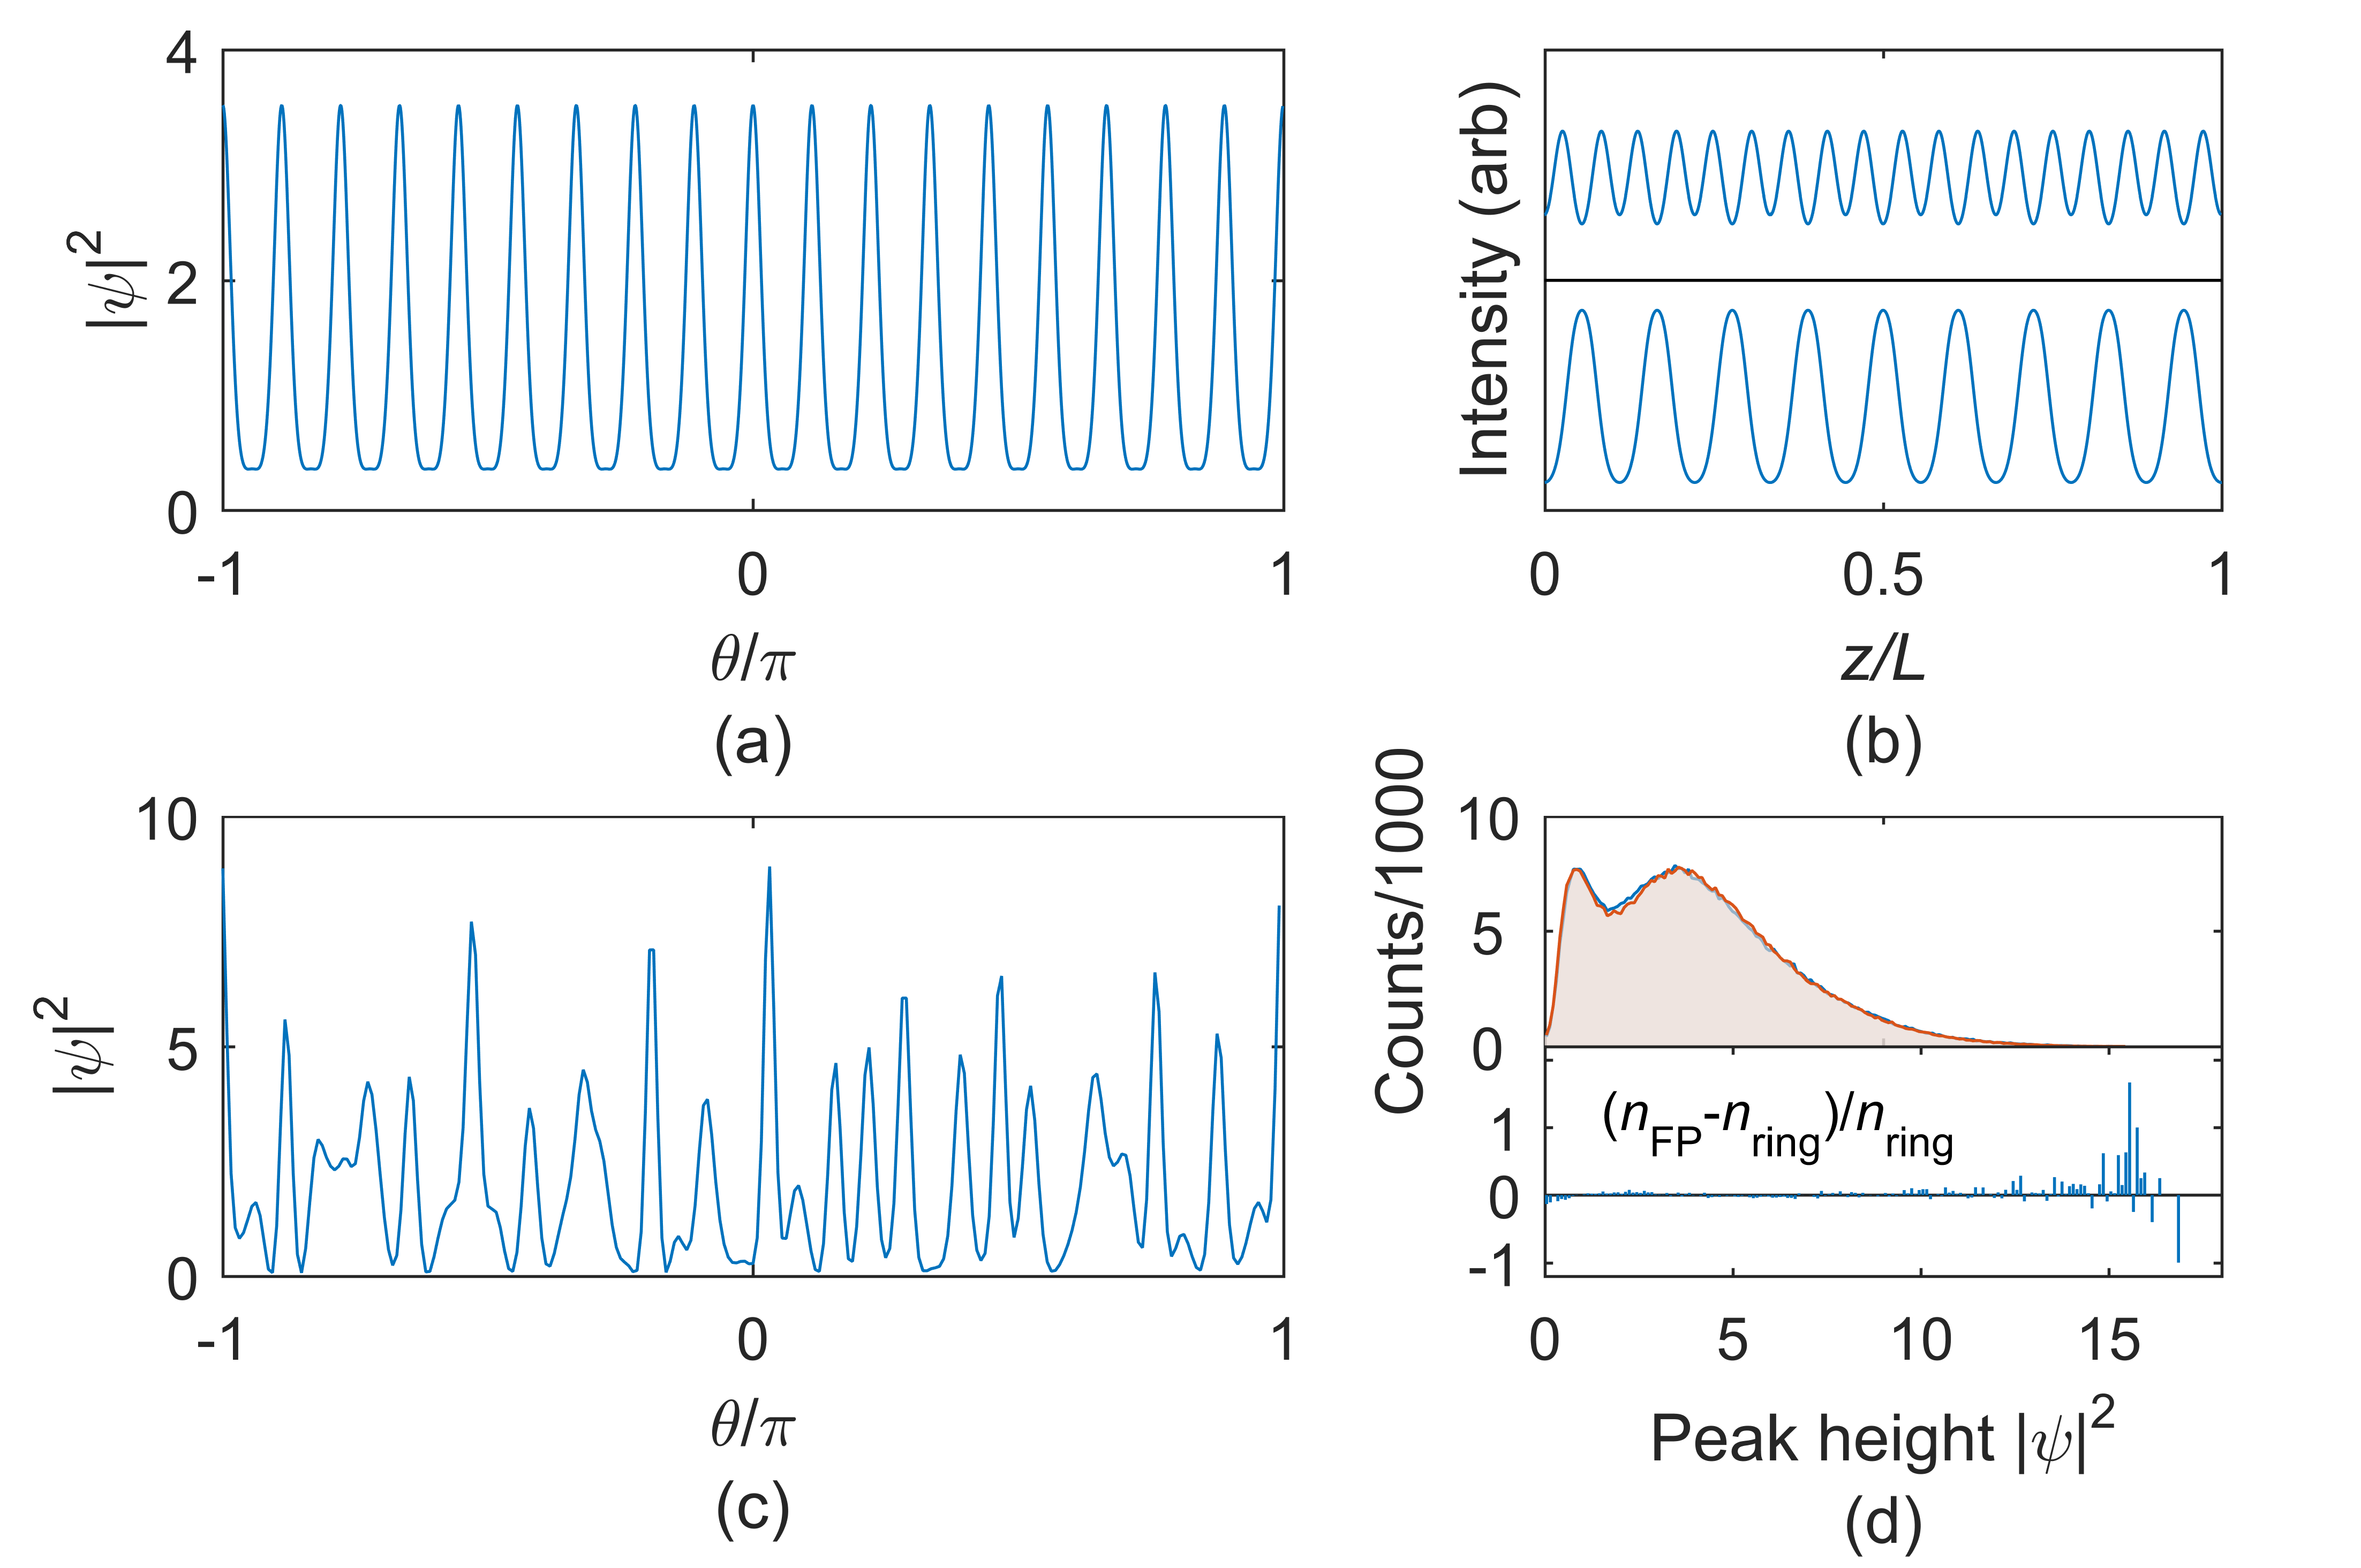
\includegraphics[]{\FigPath/Figures/FPLLE/FPLLEextendedpatterns.png}
	\end{center}
	\caption[Extended patterns in the FP-LLE]{\textbf{Extended patterns in the FP-LLE.} (a) A Turing pattern simulated at the point $(\alpha=2.5,F^2=6)$ with $\beta=-0.02$. (b) Physical intensity pattern in the cavity corresponding to to the Turing pattern shown in (a) at two different times. As $F_F$ and $F_B$ evolve, the number and positions of the local maxima change. (c) Snapshot of chaos simulated at the point $(\alpha=5.3,F^2=8)$ with $\beta=-0.02$. (d) Top: Histogram of the local maxima values in $\psi$ over a simulation of chaos at the point $(\alpha=5.3,F^2=8)$ with $\beta=-0.02$ for ten thousand photon lifetimes (blue) and at the corresponding point for the ring LLE (orange). Bottom: Fractional difference between the two histograms.}
	\label{fig:FPLLEextendedpatterns}
\end{figure} 

\section{Solitons in the FP-LLE}


\subsection{Analytical approximation for solitons in the FP-LLE}
Equipped with the definition $\alpha'=\alpha-2<|\psi|^2>$ and the relation given in Eq. \ref{eq:FPLLEaprel}, we can investigate the soliton solutions to the FP-LLE. We can immediately adapt the analytical approximation to the soliton solution for the ring LLE, which we recall here for convenience, indicating parameters defined by the detuning for the ring LLE with the `prime' superscript as in $\alpha'$:
\begin{equation}
\psi_{sol}=\psi_{CW,min}'+e^{i\phi_0'}\sqrt{2\alpha'}\,\mathrm{sech}\sqrt{\frac{2\alpha'}{-\beta_2}}\theta. \label{eq:LLEsolitonFP}
\end{equation}
Here $\psi_{CW,min}'$ is the flat solution to the ring LLE from Eq. \ref{eq:LLEflatsoln} at the point where the soliton solution is desired; when multiple flat solutions exist, $\psi_{CW,min}'$ is the one corresponding to the smallest intensity $\rho_1'$ found by solving $F^2=(1+(\alpha'-\rho')^2)\rho'$. The phase $\phi_0'$ is again defined as $\phi_0'=\mathrm{cos}^{-1}(\sqrt{8\alpha'}/\pi F)$. Thus, an approximate soliton solution to the ring LLE according to Eq. \ref{eq:LLEsolitonFP} is also an approximate soliton solution to the FP-LLE at the detuning $\alpha$, where:
\begin{align}
\alpha&=\alpha'+\frac{1}{\pi}\int d\theta |\psi_{sol}|^2\\
&=\alpha'+2\rho_1'+\frac{2}{\pi}\sqrt{-2\alpha'\beta_2}\tanh{\left(\pi\sqrt{\frac{2\alpha'}{-\beta_2}}\right)}\label{eq:FPLLEsol}\\
&\quad\quad +\frac{8}{\pi}\sqrt{-\beta_2 \rho_1'}\cos(\phi'-\phi_0')\mathrm{tan}^{-1}\tanh{\left(\pi\sqrt{\frac{\alpha'}{-2\beta_2}}\right)}\nonumber
\end{align}
and $\phi'=\mathrm{tan}^{-1}(\rho_1'-\alpha')$. To find the approximate soliton solution to the FP-LLE at a point $(\alpha,F^2)$, Eq. \ref{eq:FPLLEsol} must be numerically inverted to find $\alpha'$, after which $\psi_{sol}$ can be obtained. As is the case for the ring LLE, an approximation to multi-soliton ensembles is possible as:
\begin{equation}
\psi_{ens}=\psi_{CW,min}'+\sqrt{2\alpha^\prime}e^{i\phi_o^\prime}\sum_{j}\sech{\left(\sqrt{\frac{2\alpha^\prime}{-\beta_2}}(\theta-\theta_j)\right)}.\label{eq:FPLLEsolensemble}
\end{equation}
Such an ensemble may or may not be stable, depending on the separation between the locations of the solitons $\{\theta_j\}$ and the temporal width of the solitons determined by $\alpha'$ and $\beta_2$. Each soliton in the ensemble contributes to the average intensity $<|\psi|^2>$, so Eq. \ref{eq:FPLLEsol} no longer holds; instead, Eq. \ref{eq:FPLLEsolensemble} must be integrated to determine a new value for $\alpha'$. 

%\section{Effects of the cross-phase modulation term on solitons}
%
%In this section we discuss implications of the differences between the FP-LLE and the ring LLE\textemdash namely, the additional nonlinear integral term representing modulation by twice the average intensity\textemdash for the types of experiments that have been conducted in Kerr ring resonators. Many of the promising potential applications of c.w.-pumped Kerr ring and FP resonators rely on the generation of single solitons, so we focus here on two issues: the effect of the nonlinear integral term on the existence range of single solitons, and its effect on the experimental generation of single solitons via scans of the pump-laser frequency. These results are summarized in Fig. \ref{Fig7}. 

%\begin{figure}[]
%	\includegraphics{Fig8vector.eps} %
%	\caption{Effects of nonlinear integral term in the FP-LLE, Eq. (\ref{FPLLE}). (a) Approximate existence bounds of single solitons in the zero-dispersion limit (green, furthest left) and for $\beta=-0.001$ (blue, second from left), $\beta=-0.02$ (purple, third), and $\beta=-0.3$ (red, furthest right), calculated using the analytical approximation to the single soliton. (b) Comparisons between the approximate existence bounds and the bounds as determined numerically. Solid points indicate the maximum and minimum values of $F^2$ at which solitons have been simulated for a given value of $\alpha$. Values for the dispersion parameters are as shown in (a): $\beta=-0.001$ (blue, top), $\beta=-0.02$ (purple, middle), and $\beta=-0.3$ (red, bottom). (c) Simulated spatiotemporal chaos (blue, extended pattern) and single soliton solution (purple, localized near $\theta=0$), either of which can exist at the point $(\alpha=8,F^2=8)$. The amplitude of the soliton is larger than the characteristic amplitude of the features in the chaos because the effective detuning $\alpha^\prime$ is larger for the soliton. (d) Analytical and numerical soliton existence limits (purple) for $\beta=-0.02$ from panel (a) and the upper bound in $\alpha$ for the existence of spatiotemporal chaos/Turing patterns (black with error bars), estimated as described in the text. \label{Fig7}}
%\end{figure}

\subsection{Existence range of single solitons}
A significant consequence of the additional nonlinear term $2i\psi\left<|\psi|^2\right>$ in the FP-LLE is that the range of parameters over which single solitons exist acquires a dependence on the dispersion parameter $\beta_2$, through the effect of dispersion on pulse energy.  This is in contrast to the situation for the ring LLE, where the existence range is independent of $\beta_2$. For the FP-LLE the existence range also depends on the number of co-propagating pulses and can be greatly extended in the case of many co-propagating solitons; this is not our focus here.

The minimum value of detuning $\alpha$ at which solitons exist as a function of $F^2$ is determined by the existence of a stable flat solution to the LLE that can form the CW background for the soliton. The maximum value of detuning for which solitons can exist is determined by $\alpha^\prime=\alpha-2\left<|\psi|^2\right>$ according to $\alpha_{max}'(F^2)=\pi^2 F^2/8$, which approximately gives the maximum detuning for solitons in the ring LLE \cite{Herr2014}. 

For the FP-LLE, a stable flat solution exists to the right of the line $F_+^2 (\alpha)$ in the $\alpha-F^2$ plane that bounds the region of multiple flat solutions from above. As we did for the ring LLE, we calculate this line by beginning from the equation describing intensity of the flat stationary solutions $\rho$ to the FP-LLE:
\begin{equation}
F^2=(1+(\alpha-3\rho)^2)\rho. \label{eq:FPLLEstat2}
\end{equation} 
There are multiple flat solutions between the values $\rho_\pm$ at which $\partial F^2/\partial\rho=0$; the upper boundary of this region $F_+^2 (\alpha)$ is obtained by inserting $\rho_-=(2\alpha-\sqrt{\alpha^2-3})/9)$ into Eq. \ref{eq:FPLLEstat2}:
\begin{equation}
F_+^2 (\alpha)=\left[1+\left(\frac{\alpha+\sqrt{\alpha^2-3}}{3}\right)^2\right]\frac{2\alpha-\sqrt{\alpha^2-3}}{9}
\end{equation}
This curve bounds the region of soliton existence on the left (lower $\alpha$) in the limit $\beta_2\rightarrow0^-$ ($\beta_2$ goes to zero from below), which corresponds to the limit of zero soliton energy. In the same limit, the right boundary of soliton existence (higher $\alpha$) is the line $\alpha_{max}(F^2)=\alpha_{max}'(F^2)+2\rho_1'(\alpha_{max}'(F^2),F^2)$, where $\rho_1'(\alpha',F^2)$ is the intensity of the smallest flat solution to the ring LLE at $(\alpha',F^2)$.

We can obtain approximations to the bounds of soliton existence for finite $\beta_2$ by first finding the amplitudes $\rho_{L}(F^2)$ and $\rho_{R}(F^2)$ of the soliton background for the left and right boundaries of soliton existence in the zero-dispersion limit and then using Eq. \ref{eq:FPLLEsol} to calculate the value of $\alpha$ at which a soliton exists on a background of that amplitude for finite $\beta_2$. This process amounts to taking the amplitude of the background as an indication of the effective detuning under which the soliton evolves. These results are summarized in Fig. \ref{fig:FPLLEsolrange}. Fig. \ref{fig:FPLLEsolrange}a shows the curves corresponding to the $\beta_2\rightarrow0^-$ limit and for finite $\beta_2$ values of -0.001, -0.02, and -0.3, and Fig. \ref{fig:FPLLEsolrange}b shows a comparison between the approximate curves for finite $\beta_2$ and the soliton existence boundaries as revealed by full simulations of the FP-LLE. The analytical approximation is accurate for low $F^2$ and small dispersion, but becomes less accurate as these quantities increase. This is because breather solitons whose amplitudes oscillate periodically are found near $\alpha_{min}$ for larger values of $F^2$. Breather solitons are accompanied by traveling waves that propagate away from the soliton and diminish in amplitude as they do so, and their range increases with the dispersion. For larger values of dispersion these waves fill the cavity, and in this case the flat background whose stability forms the basis for approximating the dispersion-dependent boundary curves is actually not present. 

\begin{figure}[htpb]
	\begin{center}
		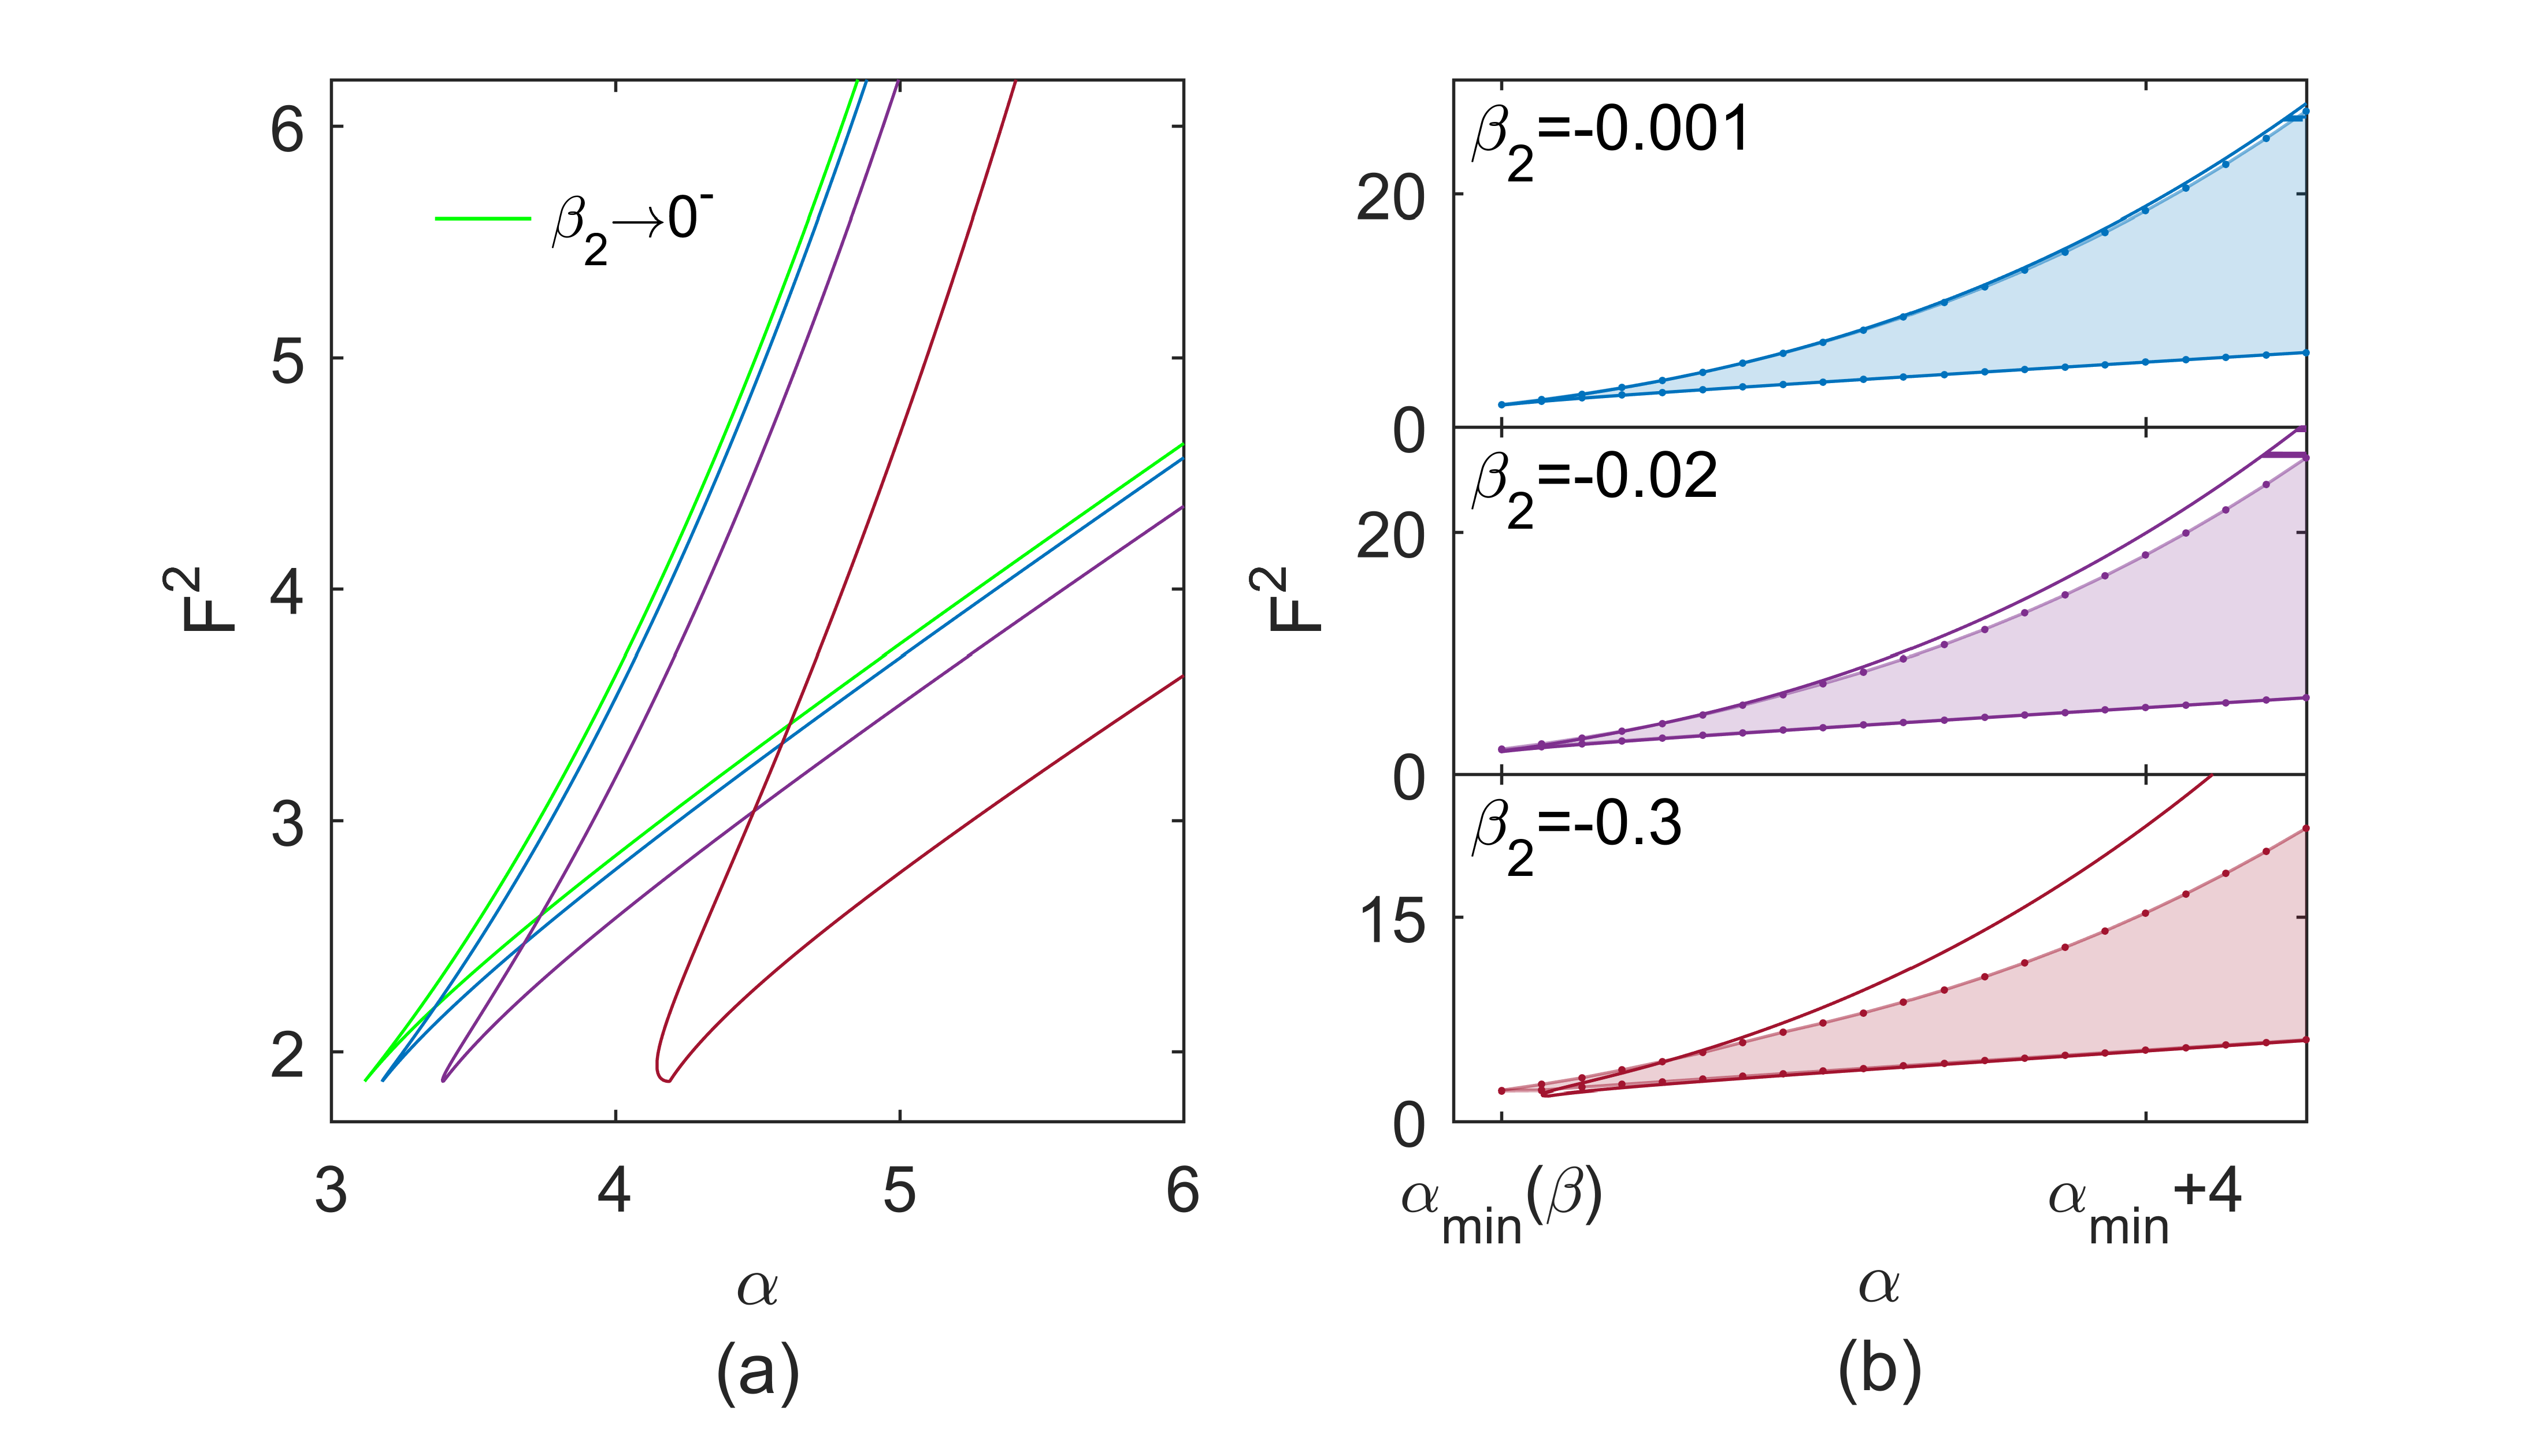
\includegraphics[]{\FigPath/Figures/FPLLE/FPLLEsolexistencerange.png}
	\end{center}
	\caption[Boundaries of soliton existence in the FP-LLE]{\textbf{Boundaries of soliton existence in the FP-LLE.} (a)~Exact boundary of soliton existence for the limit $\beta_2\rightarrow0^-$ and analytical approximations to the boundaries for three finite values of dispersion: $\beta_2=-0.001$ (blue), $\beta_2=-0.02$ (purple), and $\beta_2=-0.3$ (red). (b) Comparison between the finite-dispersion approximations from (a) and soliton existence boundaries as revealed by full simulations of the FP-LLE.  }
	\label{fig:FPLLEsolrange}
\end{figure} 

The lines $\alpha_{min} (F^2)$ and $\alpha_{max} (F^2)$ intersect at $F^2=F_I^2\approx1.87$. Below this value of the pump power solitons do not exist for the FP-LLE, and this can be seen as follows: The value of $\rho_{min}^\prime$ describing the amplitude of the soliton background along the line of maximum detuning $\alpha_{max}^\prime$ for the ring LLE is in general also a flat solution $\rho$ of the FP-LLE at the corresponding point $\alpha_{max}=\alpha_{max}^\prime+2\rho_{min}^\prime (\alpha_{max}^\prime,F^2)$. However, when $F^2<F_I^2\approx1.87$, the flat solution $\rho_{min}^\prime$ to the ring LLE is not the smallest flat solution to the FP-LLE; instead, it is the middle of three, and is therefore unstable. Therefore, when $F^2<F_I^2$ the line $\alpha_{max} (F^2)$ as defined above does not represent the right boundary of soliton existence for the FP-LLE. In fact, below this point, for all values of $\alpha$ where a stable flat solution to the FP-LLE $\rho_{min}$   exists, $\alpha-2\rho_{min} (\alpha,F^2 )>\alpha_{max}^\prime$, preventing the existence of solitons. This is an interesting contrast with the ring LLE, where the corresponding lines bounding soliton existence intersect at $F^2=1.175$ and where we can verify in simulations that solitons exist for e.g. $F^2=1.5$.


\subsection{Generation of single solitons through laser frequency scans}

A second important consequence of the additional nonlinear term in the FP-LLE relative to the ring LLE is an increase in the range of $\alpha$ values, for a given value of $F^2$, at which the state of $\psi$ can be either an extended pattern (spatiotemporal chaos or Turing pattern) or a soliton/soliton ensemble. This is because the extended patterns fill the domain and, because of their higher average intensity, experience a greater nonlinear shift than lower duty-cycle single solitons or soliton ensembles due to the additional nonlinear term. Here we discuss the implications of this fact for the experimental generation of single solitons through decreasing-frequency scans of the pump laser, as discussed in Chapter \ref{chap:microresonators}, Sec. \ref{sec:LLEsolitons}. We summarize the results in Fig. \ref{fig:FPLLE_C2S}.  In Fig. \ref{fig:FPLLE_C2S}a we show example simulations of spatiotemporal chaos and a single soliton to illustrate this degeneracy. Both of these simulations are conducted at the point $(\alpha=8,F^2=8)$, and the soliton and chaos are also degenerate with a stable flat solution, with the nature of $\psi$ dependent upon the initial conditions. 

\begin{figure}[htpb]
	\begin{center}
		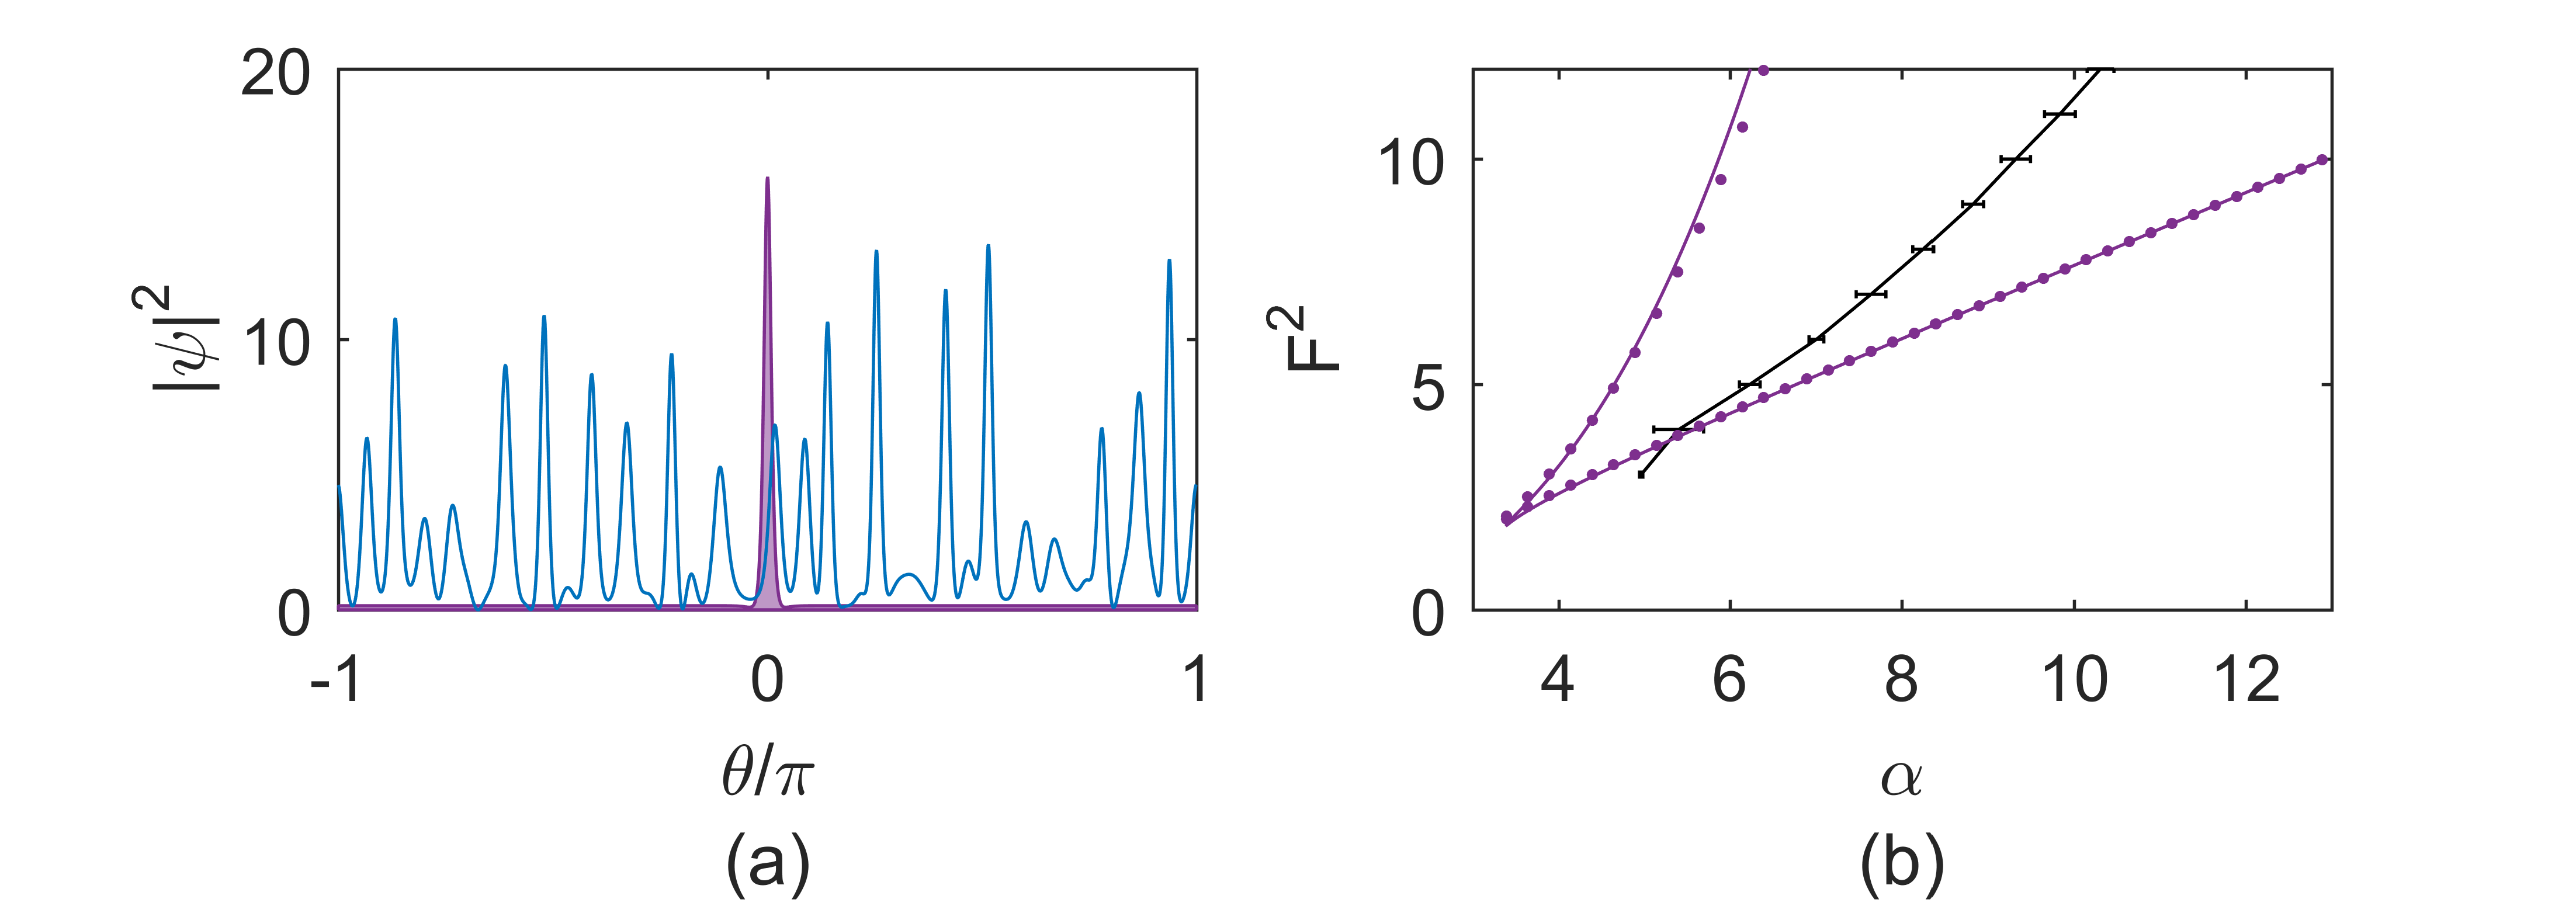
\includegraphics[]{\FigPath/Figures/FPLLE/FPLLE_C2S.png}
	\end{center}
	\caption[Transition from extended patterns to single solitons in the FP-LLE]{\textbf{Transition from extended patterns to single solitons in the FP-LLE.} (a)~Simulated spatiotemporal chaos (blue) and single soliton solution (purple), either of which can exist at the point $(\alpha=8,F^2=8)$. The amplitude of the soliton is larger than the characteristic amplitude of the features in the chaos because the effective detuning $\alpha^\prime$ is larger for the soliton. (b) Analytical (lines) and numerical (dots) soliton existence limits (purple) for $\beta=-0.02$ from panel (a) and the upper bound in $\alpha$ for the existence of spatiotemporal chaos/Turing patterns (black with error bars), estimated as described in the text. }
	\label{fig:FPLLE_C2S}
\end{figure} 

It has been established that condensation of solitons from an extended pattern in a sweep in which $\alpha$ increases is a useful way of obtaining single solitons in experiments. Because this method relies on the excitation of an extended pattern (chaos or Turing pattern) to provide initial conditions out of which solitons condense as $\alpha$ is increased, it is important that the maximum detuning (the value of $\alpha$ where $\alpha^\prime=\alpha_{max}^\prime=\pi^2 F^2/8)$ for single solitons is larger than the $\alpha$ value at which an extended pattern will transition to a soliton ensemble. Otherwise, the generation of single solitons using this method will be difficult or impossible. To investigate this, we numerically perform slow scans across the resonance to identify where the transition from extended patterns to independent solitons occurs. These scans are conducted slowly to approximate adiabaticity: $d\alpha/d\tau=2.5\times10^{-4}$. We perform $10$ scans across the resonance at each integer value of $F^2$ from $3$ to $12$ with $\beta=-0.02$, and we identify the transition from extended pattern to independent solitons by inspection of several quantities as $\alpha$ is varied: the set of local maxima and minima of $|\psi|^2$ (see Ref. \citeNoBrackets{Coillet2014}), the distance between local maxima, and the number of local maxima above $|\psi|^2=1$. In Fig. \ref{fig:FPLLE_C2S}b we plot the line representing the upper boundary in $\alpha$ of extended patterns obtained in the scans across the resonance. Error bars represent the standard deviation of the values $\alpha$ at which the transition is observed, with this spread in the values arising due to the chaotic fluctuations in the total intracavity power and therefore also in the size of the nonlinear integral term. These results indicate that the region over which single solitons exist and extended patterns do not is narrow for small pump powers $F^2$, and widens as $F^2$ is increased. Without performing experiments, it is impossible to precisely quantify the limitations imposed by this observation, but we expect this finding to be useful in refining schemes for single-soliton generation in Fabry-Perot resonators. It is important to note that challenges associated with the necessary transition from high duty-cycle extended patterns to low duty-cycle solitons are alleviated by pulsed pumping, which was the technique used by Obrzud, Lecomte, and Herr in their recent report of soliton generation in FP resonators \cite{Obrzud2017}.



